% Created 2016-02-25 Thu 20:44
\documentclass[11pt]{article}
\usepackage[utf8]{inputenc}
\usepackage{lmodern}
\usepackage[T1]{fontenc}
\usepackage{fixltx2e}
\usepackage{graphicx}
\usepackage{longtable}
\usepackage{float}
\usepackage{wrapfig}
\usepackage{rotating}
\usepackage[normalem]{ulem}
\usepackage{amsmath}
\usepackage{textcomp}
\usepackage{marvosym}
\usepackage{wasysym}
\usepackage{amssymb}
\usepackage{amsmath}
\usepackage[version=3]{mhchem}
\usepackage[numbers,super,sort&compress]{natbib}
\usepackage{natmove}
\usepackage{url}
\usepackage{minted}
\usepackage{underscore}
\usepackage[linktocpage,pdfstartview=FitH,colorlinks,
linkcolor=blue,anchorcolor=blue,
citecolor=blue,filecolor=blue,menucolor=blue,urlcolor=blue]{hyperref}
\usepackage{attachfile}
\usepackage{graphicx}
\usepackage{subfigure}
\usepackage{pdfcomment}
\date{\today}
\title{blog}
\begin{document}

\section{Adding captions and attributes to figures and tables from code blocks}
\label{sec-1}

I have wanted for a long time to be able to add captions and attributes to figures and tables generated from code blocks. I brought this up on the mailing list (\url{https://lists.gnu.org/archive/html/emacs-orgmode/2015-11/msg00544.html}) and finally, I have figured out a way to do it that seems ok. It is based on the :wrap feature of org-babel.

The idea is to use a function that will wrap the results in additional text. We use this function that will add a caption and attributes.

\begin{minted}[frame=lines,fontsize=\scriptsize,linenos]{common-lisp}
(defun decorate-org-results (&optional caption attributes)
  "A wrap function for src blocks."
  (concat
   "ORG\n"
   (when attributes
     (concat (mapconcat 'identity attributes "\n") "\n"))
   (when caption
     (format "#+caption: %s" caption))))
\end{minted}

\begin{verbatim}
decorate-org-results
\end{verbatim}

Now, we try it out on a figure:

\begin{minted}[frame=lines,fontsize=\scriptsize,linenos]{python}
import numpy as np
import matplotlib.pyplot as plt

x = np.linspace(0, 2 * np.pi)
y = np.sin(x)

plt.plot(x, y)
plt.savefig('images/sin.png')
print('[[./images/sin.png' + ']]')
\end{minted}

\begin{org}
\begin{figure}[htb]
\centering
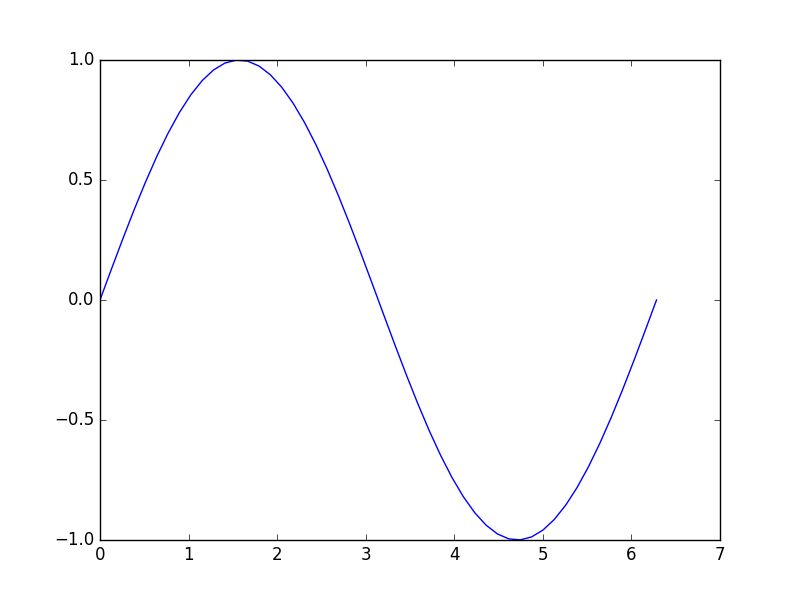
\includegraphics[width=3in]{./images/sin.png}
\caption{A sin wave. \label{fig-sin}}
\end{figure}
\end{org}

Success. Next, on a table.

\begin{minted}[frame=lines,fontsize=\scriptsize,linenos]{python}
import numpy as np

x = np.linspace(0, 2 * np.pi, 5)
y = np.sin(x)

return [['x', 'y'], None] + list(zip(x, y))
\end{minted}

\begin{org}
\begin{table}[H]
\caption{A table of sin data. \label{tab-sin}}
\centering
\begin{tabular}{rr}
x & y\\
\hline
0.0 & 0.0\\
1.5707963267948966 & 1.0\\
3.141592653589793 & 1.2246467991473532\,(-16)\\
4.71238898038469 & -1.0\\
6.283185307179586 & -2.4492935982947064\,(-16)\\
\end{tabular}
\end{table}
\end{org}
% Emacs 25.1.50.1 (Org mode 8.2.10)
\end{document}